\documentclass[presentation]{beamer}

\usepackage[utf8]{inputenc}
% \usepackage[T1]{fontenc}
\usepackage{fixltx2e}
\usepackage{graphicx}
% \usepackage{longtable}
% \usepackage{tabu}
\usepackage{makecell}
\usepackage{float}
\usepackage{subcaption}
\usepackage{wrapfig}
\usepackage{rotating}
\usepackage[normalem]{ulem}
\usepackage{amsmath}
% \usepackage{textcomp}
% \usepackage{marvosym}
% \usepackage{wasysym}
% \usepackage{amssymb}
\usepackage{hyperref}
\usepackage{ragged2e}
\usepackage{xcolor}


\usepackage{bm}

\usepackage{amsmath,amssymb}
\newcommand{\bx}{\mathbf{x}}
\newcommand{\bv}{\mathbf{v}}
\newcommand{\bp}{\mathbf{p}}
\newcommand{\bq}{\mathbf{q}}
\newcommand{\by}{\mathbf{y}}

\newcommand{\bbR}{\mathbb{R}}
\newcommand{\bbN}{\mathbb{N}}

\newcommand{\bxi}{\bm{\xi}}
\newcommand{\bal}{\bm{\alpha}}
\newcommand{\bth}{\bm{\theta}}

\usepackage{etoolbox}
\let\bbordermatrix\bordermatrix
\patchcmd{\bbordermatrix}{8.75}{4.75}{}{}
\patchcmd{\bbordermatrix}{\left(}{\left[}{}{}
\patchcmd{\bbordermatrix}{\right)}{\right]}{}{}

\usepackage[authoryear, round]{natbib}

\newcommand{\sidebysidecaption}[4]{%
\RaggedRight%
  \begin{minipage}[t]{#1}
    \vspace*{0pt}
    #3
  \end{minipage}
  \hfill%
  \begin{minipage}[t]{#2}
    \vspace*{0pt}
    #4
\end{minipage}%
}

%% colors
\definecolor{Red}{rgb}{0.7,0,0}
\definecolor{Blue}{rgb}{0,0,0.8}
\definecolor{Green}{rgb}{0,0.8,0}
\definecolor{Gray}{rgb}{0.8,0.8,0.8}
\definecolor{Orange}{rgb}{1,.65,0}

\usepackage{hyperref}
\hypersetup{
  hyperindex = {true},
  colorlinks = {true},
  linktocpage = {true},
  plainpages = {false},
  linkcolor = {Blue},
  citecolor = {Blue},
  urlcolor = {Red},
  pdfstartview = {Fit},
  pdfpagemode = {UseOutlines},
  pdfview = {XYZ null null null},
  pdfkeywords={proteomics, spatial, dynamics, integration, regulation, computational biology},
  pdfsubject={Research talk},
  pdfcreator={Laurent Gatto}}

%% knitr

%% maxwidth is the original width if it is less than linewidth
%% otherwise use linewidth (to make sure the graphics do not exceed the margin)
\makeatletter
\def\maxwidth{ %
  \ifdim\Gin@nat@width>\linewidth
    \linewidth
  \else
    \Gin@nat@width
  \fi
}
\makeatother

\definecolor{fgcolor}{rgb}{0.345, 0.345, 0.345}
\newcommand{\hlnum}[1]{\textcolor[rgb]{0.686,0.059,0.569}{#1}}%
\newcommand{\hlstr}[1]{\textcolor[rgb]{0.192,0.494,0.8}{#1}}%
\newcommand{\hlcom}[1]{\textcolor[rgb]{0.678,0.584,0.686}{\textit{#1}}}%
\newcommand{\hlopt}[1]{\textcolor[rgb]{0,0,0}{#1}}%
\newcommand{\hlstd}[1]{\textcolor[rgb]{0.345,0.345,0.345}{#1}}%
\newcommand{\hlkwa}[1]{\textcolor[rgb]{0.161,0.373,0.58}{\textbf{#1}}}%
\newcommand{\hlkwb}[1]{\textcolor[rgb]{0.69,0.353,0.396}{#1}}%
\newcommand{\hlkwc}[1]{\textcolor[rgb]{0.333,0.667,0.333}{#1}}%
\newcommand{\hlkwd}[1]{\textcolor[rgb]{0.737,0.353,0.396}{\textbf{#1}}}%

\usepackage{framed}
\makeatletter
\newenvironment{kframe}{%
 \def\at@end@of@kframe{}%
 \ifinner\ifhmode%
  \def\at@end@of@kframe{\end{minipage}}%
  \begin{minipage}{\columnwidth}%
 \fi\fi%
 \def\FrameCommand##1{\hskip\@totalleftmargin \hskip-\fboxsep
 \colorbox{shadecolor}{##1}\hskip-\fboxsep
     % There is no \\@totalrightmargin, so:
     \hskip-\linewidth \hskip-\@totalleftmargin \hskip\columnwidth}%
 \MakeFramed {\advance\hsize-\width
   \@totalleftmargin\z@ \linewidth\hsize
   \@setminipage}}%
 {\par\unskip\endMakeFramed%
 \at@end@of@kframe}
\makeatother

\definecolor{shadecolor}{rgb}{.97, .97, .97}
\definecolor{messagecolor}{rgb}{0, 0, 0}
\definecolor{warningcolor}{rgb}{1, 0, 1}

\definecolor{errorcolor}{rgb}{1, 0, 0}
\newenvironment{knitrout}{}{} % an empty environment to be redefined in TeX

\usepackage{alltt}
\usepackage[utf8]{inputenc}
\usepackage[T1]{fontenc}
\usepackage{fixltx2e}
\usepackage{graphicx}
\usepackage{longtable}
\usepackage{float}
\usepackage{wrapfig}
\usepackage{rotating}
\usepackage[normalem]{ulem}
\usepackage{amsmath}
\usepackage{textcomp}
\usepackage{marvosym}
\usepackage{wasysym}
\usepackage{amssymb}


\date{\textbf{Protein Folding and Stability}\\
  30 August 2019 -- Li\`ege}

\title{\textbf{Mapping the sub-cellular proteome}\\
  \small{Probabilistic modelling of protein sub-cellular localisation}}

\author{Laurent Gatto\\
  \url{laurent.gatto@uclouvain.be}\\
  \url{http://lgatto.github.io/about}\\
  de Duve Institute -- UCLouvain\\
  \bigskip
  %% Slides: \url{http://bit.ly/20190718iscb}  (CC-BY)
}


\begin{document}

\maketitle


\section{Spatial proteomics}


\begin{frame}{Cell organisation - \textbf{localisation is function}}
  \begin{center}
    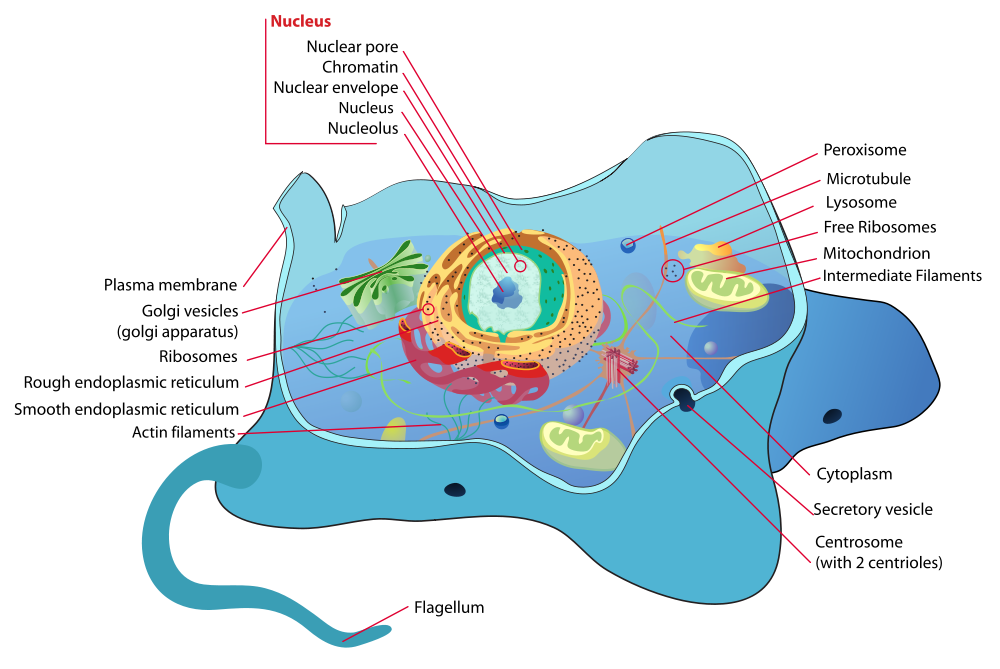
\includegraphics[width=.9\linewidth]{figs/Animal_cell_structure.png} \\
    \textbf{\textcolor{Blue}{Spatial proteomics}} is the systematic
    study of protein localisations.
  \end{center}

  \begin{center}
    \textbf{Localisation(s) -- re-localisation -- mis-localisation}
  \end{center}
  
  \tiny Image from Wikipedia
  \url{http://en.wikipedia.org/wiki/Cell_(biology)}.  
\end{frame}


%% \begin{frame}{Spatial proteomics - Why?}

%%   \begin{itemize}

%%   \item \textbf{Localisation is function}: Localisation and
%%     sequestration of proteins within sub-cellular niches is a
%%     fundamental mechanism for the post-translational regulation of
%%     protein function.

%%     \bigskip

%%   \item \textbf{Re-localisation}: \textcolor{Blue}{differentiation}
%%     stem cells, \textcolor{Blue}{activation} of biological processes.

%%     \bigskip

%%   \item \textbf{Mis-localisation}: Disruption of the
%%     targeting/trafficking process alters proper sub-cellular
%%     localisation, which in turn perturb the cellular functions of the
%%     proteins.

%%   \end{itemize}

%% \end{frame}


\begin{frame}{Fusion proteins and immunofluorescence}

  \begin{figure}[h]
    \centering
    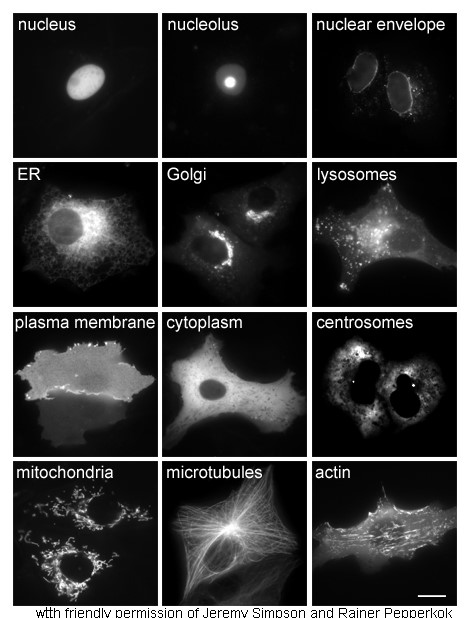
\includegraphics[width=.35\linewidth]{figs/Localisations02eng.jpg}
    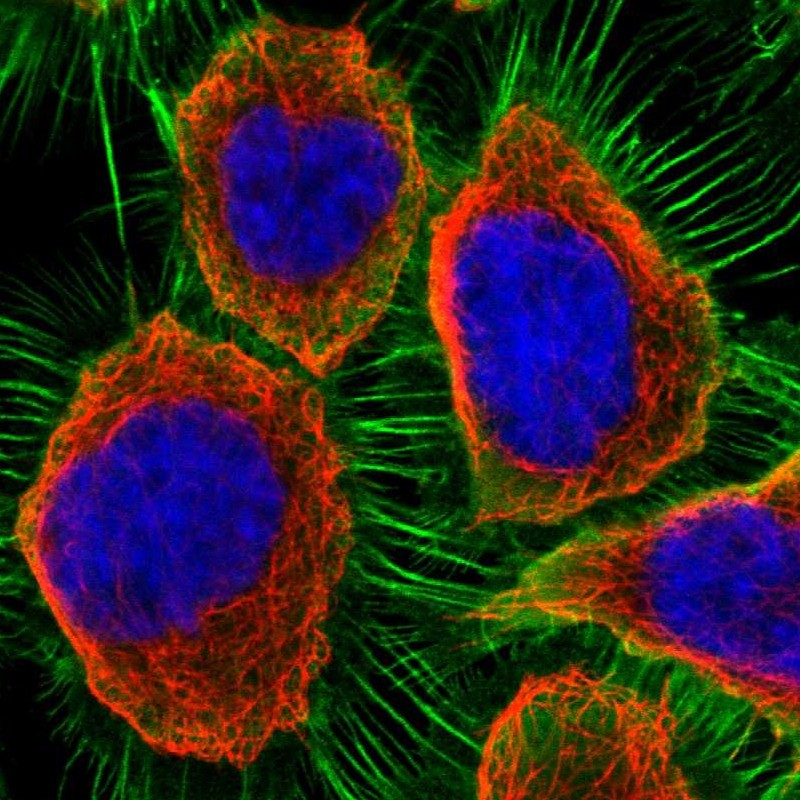
\includegraphics[width=.45\linewidth]{figs/if_selected.jpg}
    \caption{Targeted protein localisation. Example of discrepancies
      between IF and FPs as well as between FP tagging at the N and C
      termini \citep{Stadler:2013}.}
  \end{figure}
\end{frame}


\begin{frame}{}

  \begin{columns}
    \begin{column}{0.5\textwidth}

      \textbf{Explorative/discovery approaches},
      \textcolor{Blue}{steady-state \textbf{global localisation maps}}
      (as opposed to microscopy-based targeted approaches).

      \bigskip
      
      \small{

        \textbf{Density gradient}: PCP \citep{Dunkley:2006}, LOPIT
        \citep{Foster2006}, hyperLOPIT
        \citep{Christoforou:2016,Mulvey:2017} and \\

        \textbf{Differential centrifugation} \cite{Itzhak:2016},
        LOPIT-DC \citep{Geladaki:2018}.

      }
     
      \bigskip
      
      
    \end{column}
    \begin{column}{0.5\textwidth}
      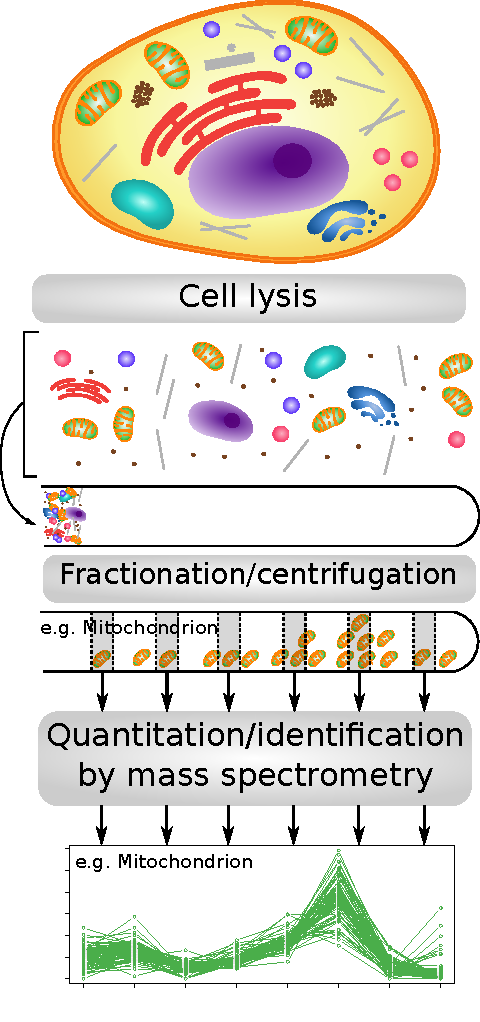
\includegraphics[width=.8\linewidth]{figs/workflow_primary.pdf}
    \end{column}    
  \end{columns}
  
\end{frame}

\subsubsection*{The data}
\label{sec:data}

\begin{frame}{Quantitation data}
  \begin{center}
    \begin{tabular}{|l|llll|}
      \hline
      & Fraction$_{\text{1}}$ & Fraction$_{\text{2}}$ & \ldots{} & Fraction$_{\text{L}}$ \\
      \hline
      {\bf x}$_{\text{1}}$ & $x_{\text{1,1}}$ & $x_{\text{1,2}}$ & \ldots{} & $x_{\text{1,L}}$ \\
      {\bf x}$_{\text{2}}$ & $x_{\text{2,1}}$ & $x_{\text{2,2}}$ & \ldots{} & $x_{\text{2,L}}$ \\
      {\bf x}$_{\text{3}}$ & $x_{\text{3,1}}$ & $x_{\text{3,2}}$ & \ldots{} & $x_{\text{3,L}}$ \\
      \vdots & \vdots & \vdots & \vdots & \vdots \\
      {\bf x}$_{\text{i}}$ & $x_{\text{i,1}}$ & $x_{\text{i,2}}$ & \ldots{} & $x_{\text{i,L}}$ \\
      \vdots & \vdots & \vdots & \vdots & \vdots \\
      {\bf x}$_{\text{N}}$ & $x_{\text{N,1}}$ & $x_{\text{N,2}}$ & \ldots{} & $x_{\text{N, L}}$ \\
      \hline
    \end{tabular}
  \end{center}
\end{frame}

\begin{frame}{Quantitation data and organelle markers}
  \begin{center}
    \begin{tabular}{|l|llll||l|}
      \hline
      & Fraction$_{\text{1}}$ & Fraction$_{\text{2}}$ & \ldots{} & Fraction$_{\text{L}}$ & markers\\
      \hline
      {\bf x}$_{\text{1}}$ & $x_{\text{1,1}}$ & $x_{\text{1,2}}$ & \ldots{} & $x_{\text{1,L}}$ & unknown \\
      {\bf x}$_{\text{2}}$ & $x_{\text{2,1}}$ & $x_{\text{2,2}}$ & \ldots{} & $x_{\text{2,L}}$ & \textcolor{Red}{$loc_{1}$}\\
      {\bf x}$_{\text{3}}$ & $x_{\text{3,1}}$ & $x_{\text{3,2}}$ & \ldots{} & $x_{\text{3,L}}$ & unknown \\
      \vdots & \vdots & \vdots & \vdots & \vdots & \vdots \\
      {\bf x}$_{\text{i}}$ & $x_{\text{i,1}}$ & $x_{\text{i,2}}$ & \ldots{} & $x_{\text{i,L}}$ & \textcolor{Blue}{$loc_{k}$}\\
      \vdots & \vdots & \vdots & \vdots & \vdots & \vdots\\
      {\bf x}$_{\text{N}}$ & $x_{\text{N,1}}$ & $x_{\text{N,2}}$ & \ldots{} & $x_{\text{N, K}}$ & unknown \\
      \hline
    \end{tabular}
  \end{center}
\end{frame}

%% \begin{frame}{}
%%   \begin{center}
%%     \Large{Data analysis}
%%   \end{center}
%% \end{frame}


\subsection*{Data analysis}
\label{sec:comp}

\subsubsection*{Visualisation}
\label{sec:viz}

\begin{frame}{Visualisation}
  \begin{figure}
    \centering
    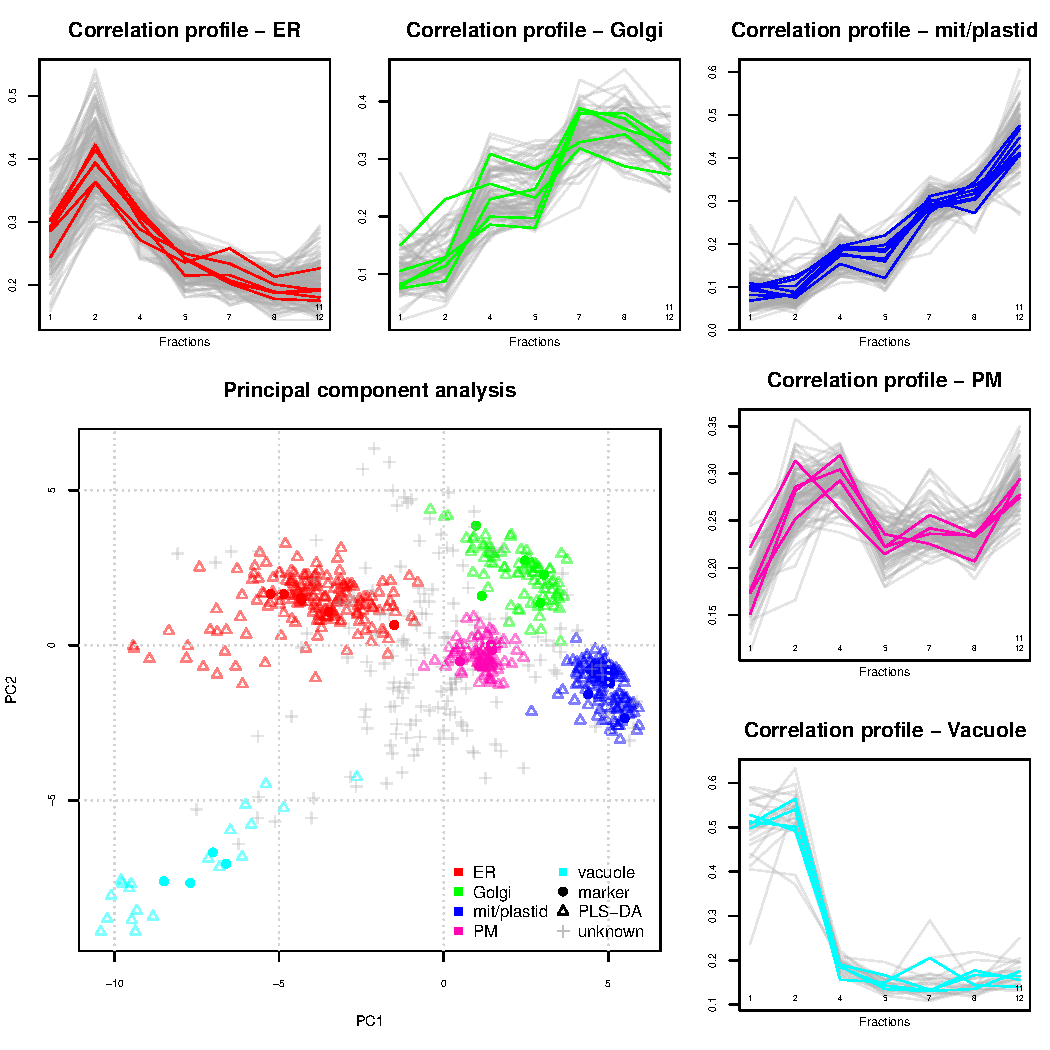
\includegraphics[width=.6\linewidth]{figs/F04-analyses.pdf}
    \caption{From \cite{Gatto:2010}, \textit{Arabidopsis thaliana} data
      from \cite{Dunkley:2006}}
  \end{figure}
\end{frame}

\subsubsection*{Machine learning}
\label{sec:ml}

\begin{frame}{Supervised Machine Learning to infer \textbf{localisation}}
  \begin{figure}[h]
    \centering
    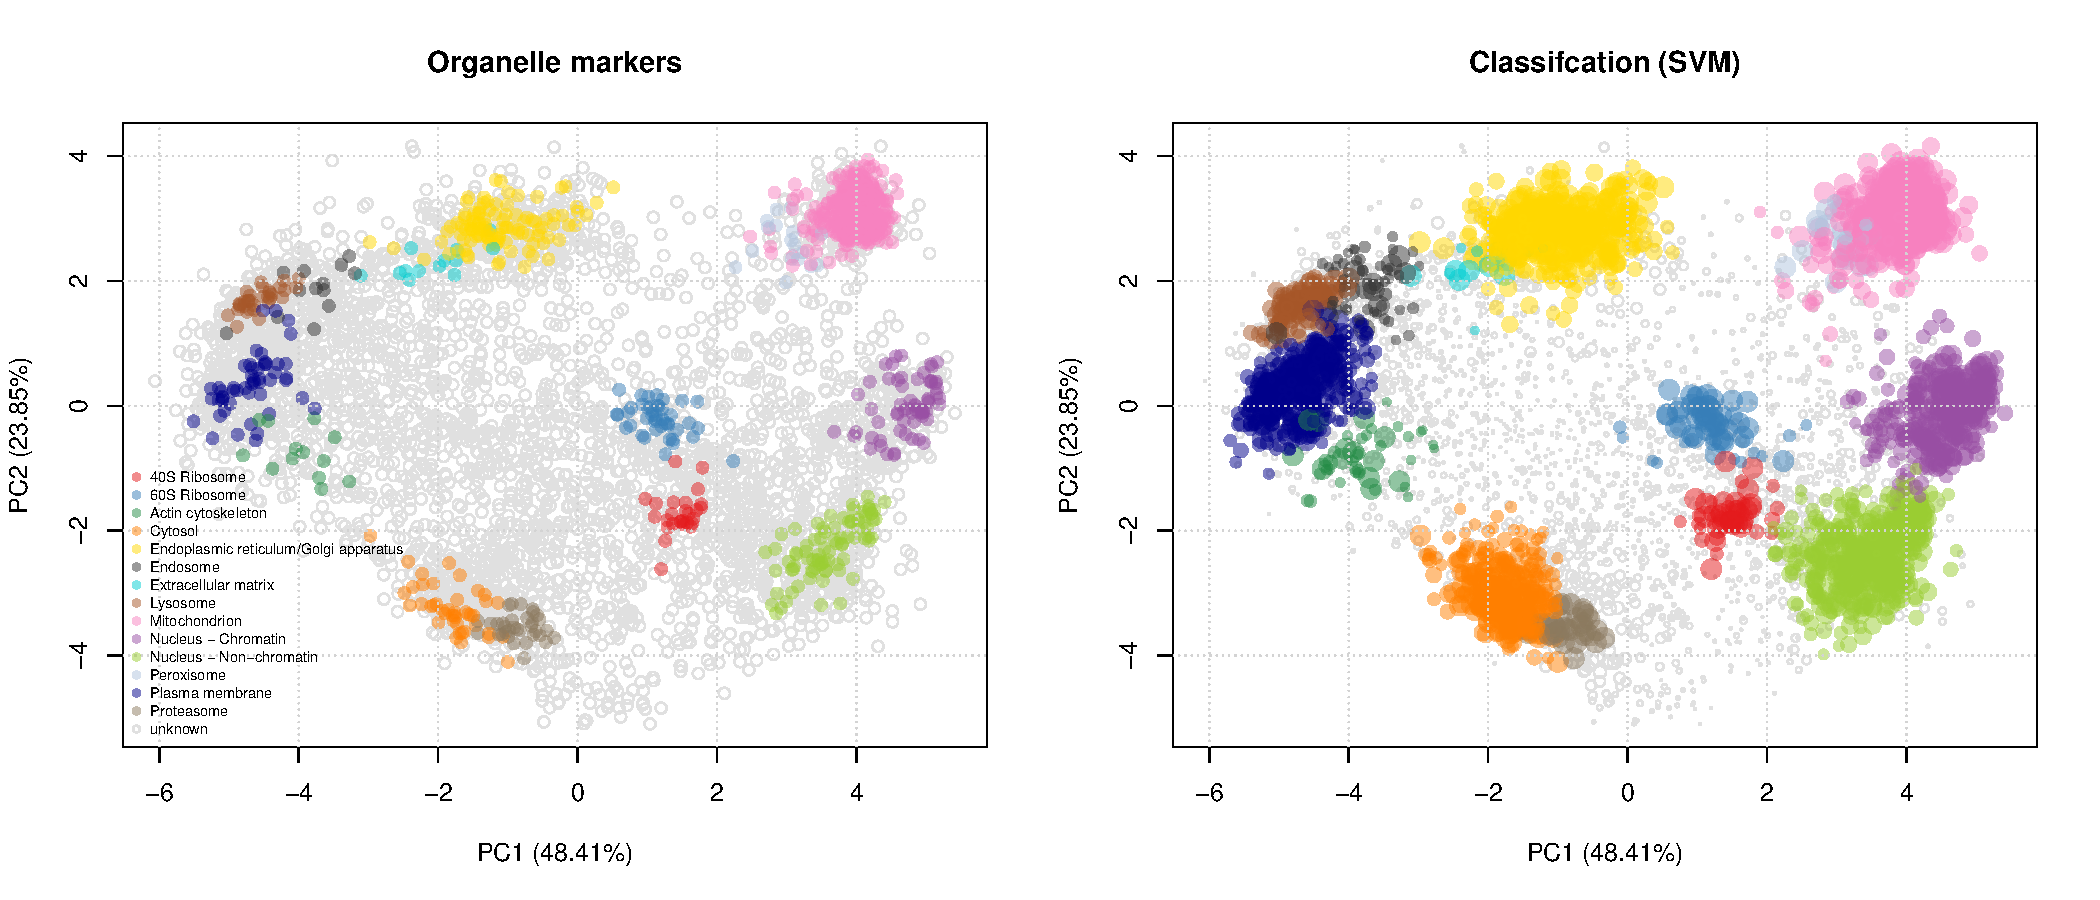
\includegraphics[width=\linewidth]{figs/hyperlopit-class.pdf}
    \caption{Support vector machines classifier (after 5\% FDR
      classification cutoff) on the embryonic stem cell data from
      \cite{Christoforou:2016}.}
  \end{figure}
\end{frame}


\subsection{Embracing uncertainty}

\begin{frame}{How much do we learn? How much do we miss?}
  \begin{figure}
    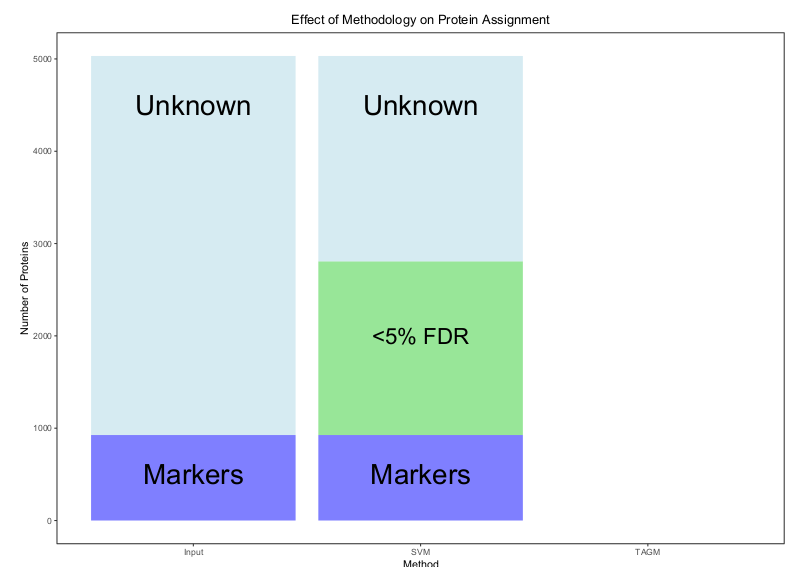
\includegraphics[width=.8\linewidth]{./figs/preConcludePlot.png}
  \end{figure}
\end{frame}



\begin{frame}{A Bayesian Mixture Modelling Approach For Spatial Proteomics}

  \begin{itemize}

    \item<+-> \textit{T Augmented Gaussian Mixture model (TAGM)} is a
      \textbf{multivariate Gaussian generative model} for MS-based
      spatial proteomics data. It posits that each annotated
      sub-cellular niche can be modelled by a multivariate Gaussian
      distribution.

    \item<+-> With the prior knowledge that many proteins are not
      captured by known sub-cellular niches, we augment our model with
      an \textbf{outlier component}. Outliers are often dispersed and
      thus this additional component is described by a heavy-tailed
      distribution: the multivariate Student's t-distribution, leading
      us to a \textit{T Augmented Gaussian Mixture model}
      \citep{Crook:2018,Crook:2019}.

    \item<+-> This methodology allows proteome-wide
      \textbf{uncertainty quantification}, thus adding a further layer
      to the analysis of spatial proteomics.

  \end{itemize}
\end{frame}


\begin{frame}{}

    We initially model the distribution of profiles associated with
    proteins that localise to the $k$-th component as multivariate
    normal with mean vector $\boldsymbol{\mu}_k$ and covariance matrix
    $\Sigma_k$, so that:

    \begin{align}
      {\bf x}_i | z_i = k \quad \sim \mathcal{N}(\boldsymbol{\mu}_k, \Sigma_k) \label{equation::preq}
    \end{align}

    \pause

    We extend it by introducing an additional \textit{outlier
      component}. To do this, we augment our model by introducing a
    further indicator latent variable $\phi$. Each protein ${\bf x}_i$
    is now described by an additional variable $\phi_i$, with $\phi_i
    = 1$ indicating that protein ${\bf x}_i$ belongs to a organelle
    derived component and $\phi_i = 0$ indicating that protein ${\bf
      x}_i$ is not well described by these known components. This
    outlier component is modelled as a multivariate T distribution
    with degrees of freedom $\kappa$, mean vector $\bf{M}$, and scale
    matrix $V$.

    \begin{align}
      {\bf x}_i | z_i = k, \phi_i \quad \sim \mathcal{N}(\boldsymbol{\mu}_k, \Sigma_k)^{\phi_i}\mathcal{T}(\kappa, \boldsymbol{M}, V)^{1 - \phi_i }
    \end{align}


\end{frame}


\begin{frame}[fragile]{}
      \begin{figure}
        \sidebysidecaption{0.65\linewidth}{0.3\linewidth}{
          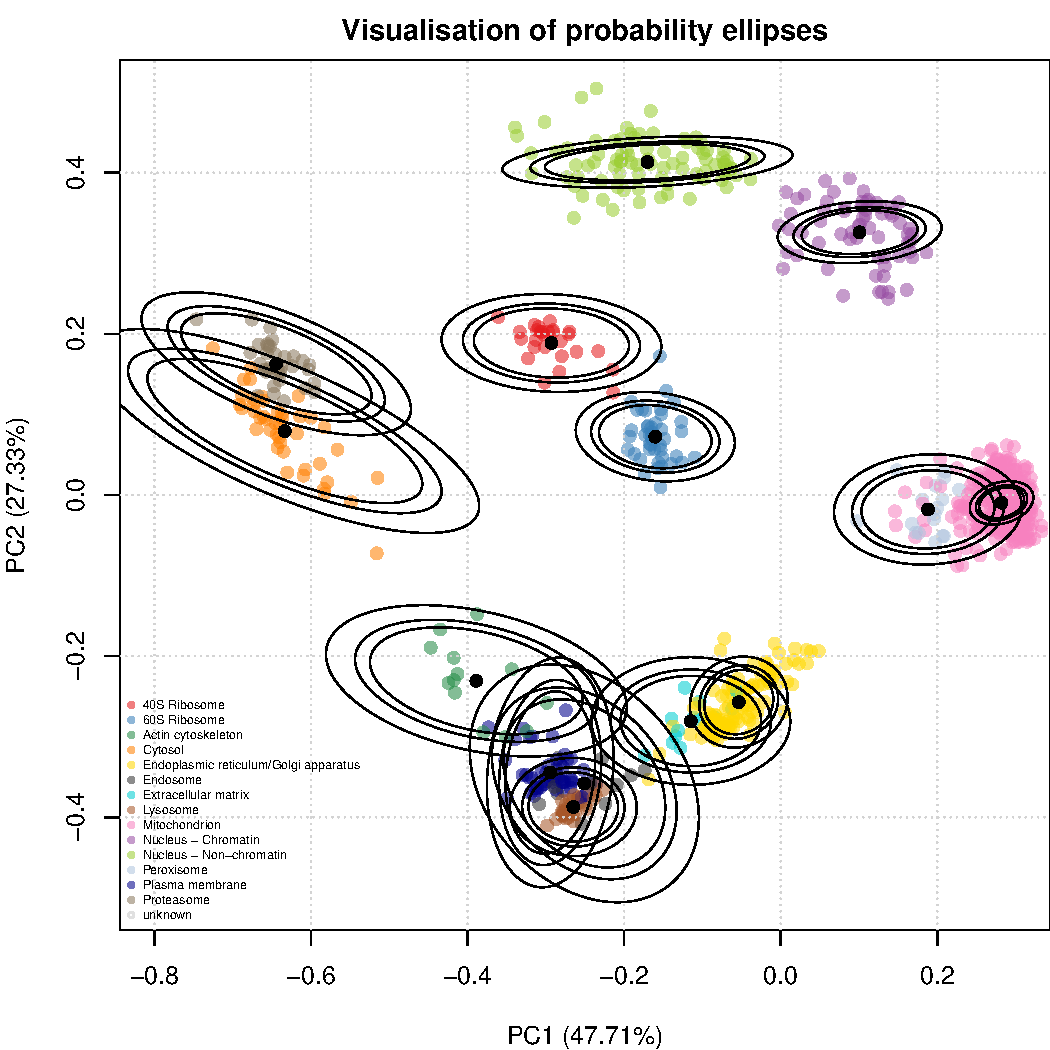
\includegraphics[width=1\linewidth]{./figs/pca12-ellipses-1.pdf}
        }{
          \caption{\scriptsize \justifying Illustration of how the
            TAGM model describes the pluripotent mouse embryonic stem
            cell data. Each ellipse contains a proportion of total
            probability of a particular multivariate Gaussian density.
            The outer ellipse contains $99\%$ of the total probability
            whilst the middle and inner ellipses contain $95\%$ and
            $90\%$ of the probability respectively.}
          \label{fig:tagm}
        }
      \end{figure}

      %% NOTE that while some sub-cellular clusters overlap along PC1 and
      %% PC2, they are separated along additional dimensions.

\end{frame}

\begin{frame}{}
      \begin{figure}
        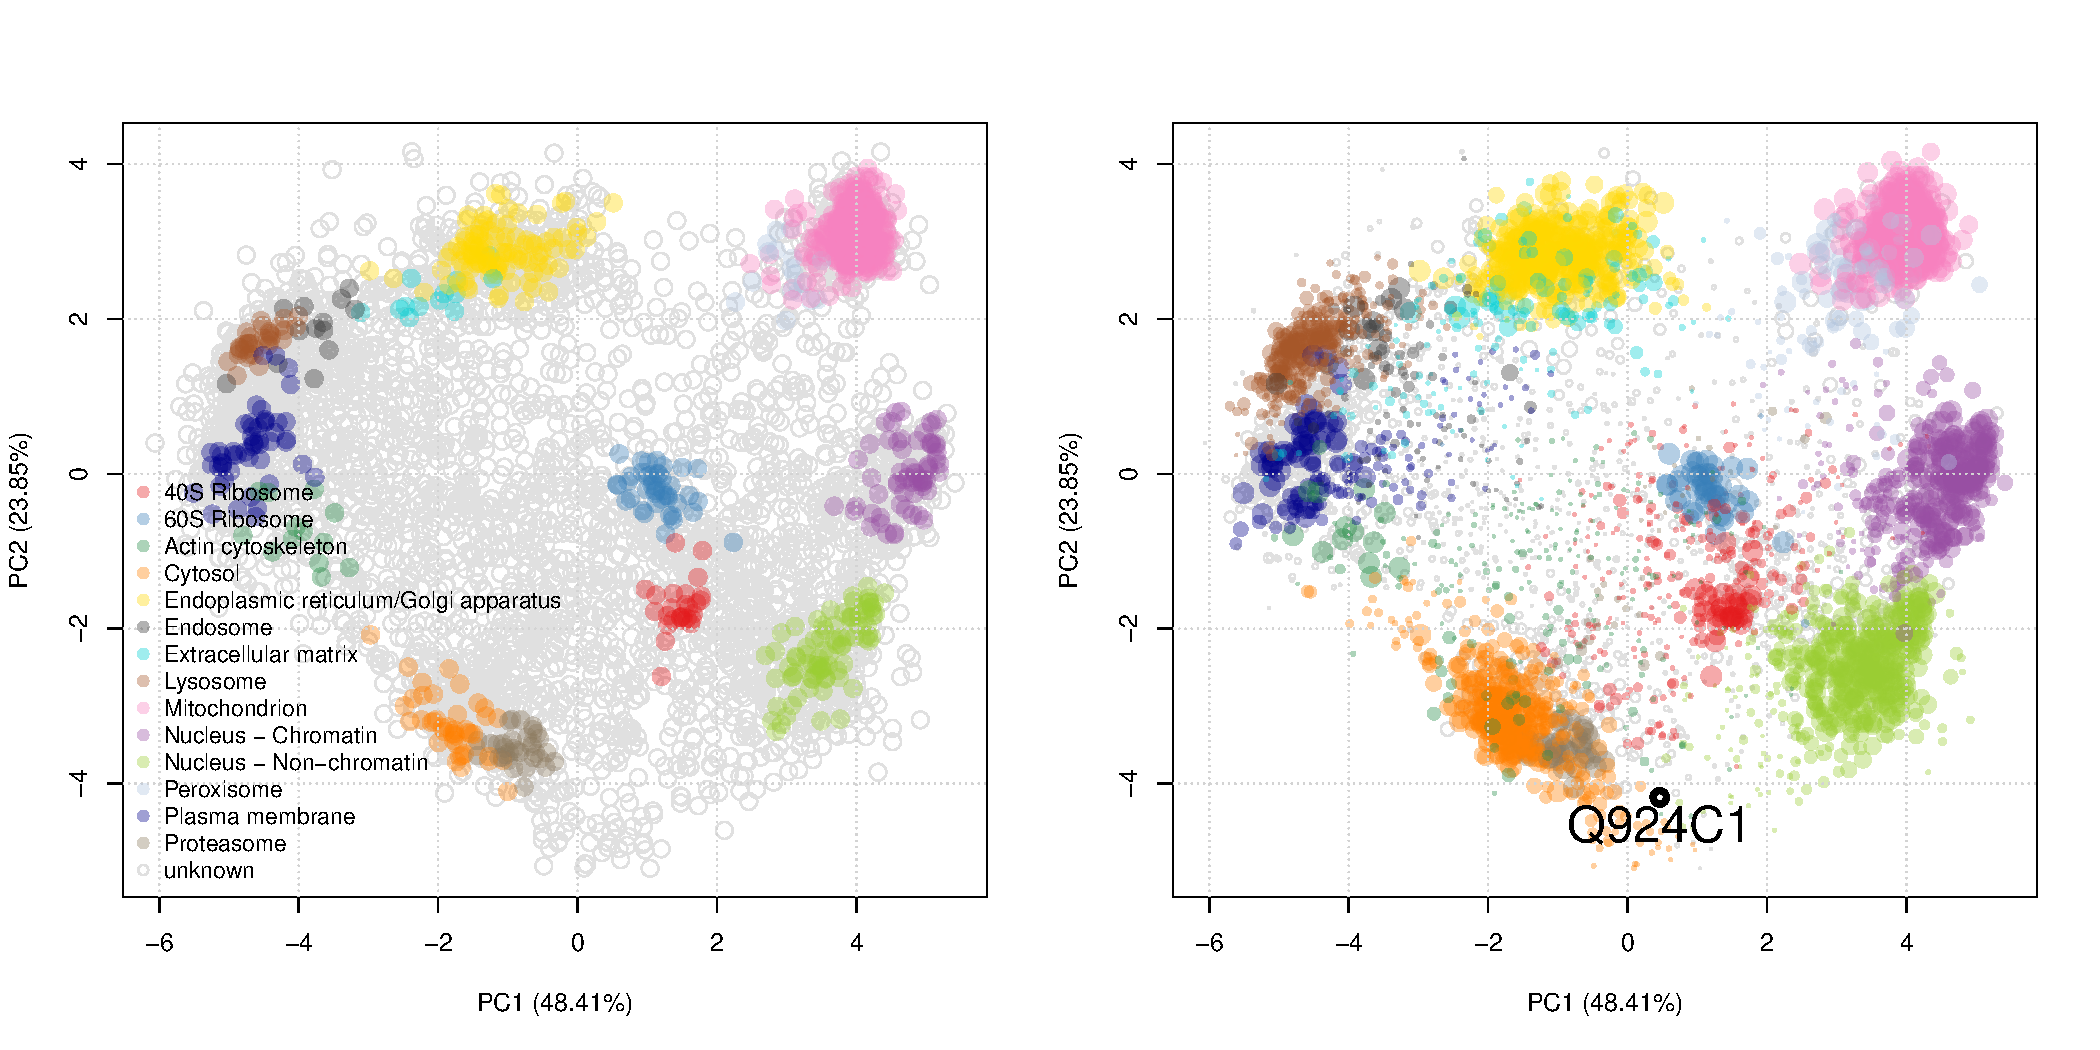
\includegraphics[width=1\linewidth]{./figs/tagm_pca_res.pdf}
        \caption{Assignment of proteins of
          \textit{unknown} location to one of the annotated
          classes. The dots are scaled according to the protein
          assignment probabilities.}
      \end{figure}
\end{frame}

\begin{frame}{}
  \begin{figure}
    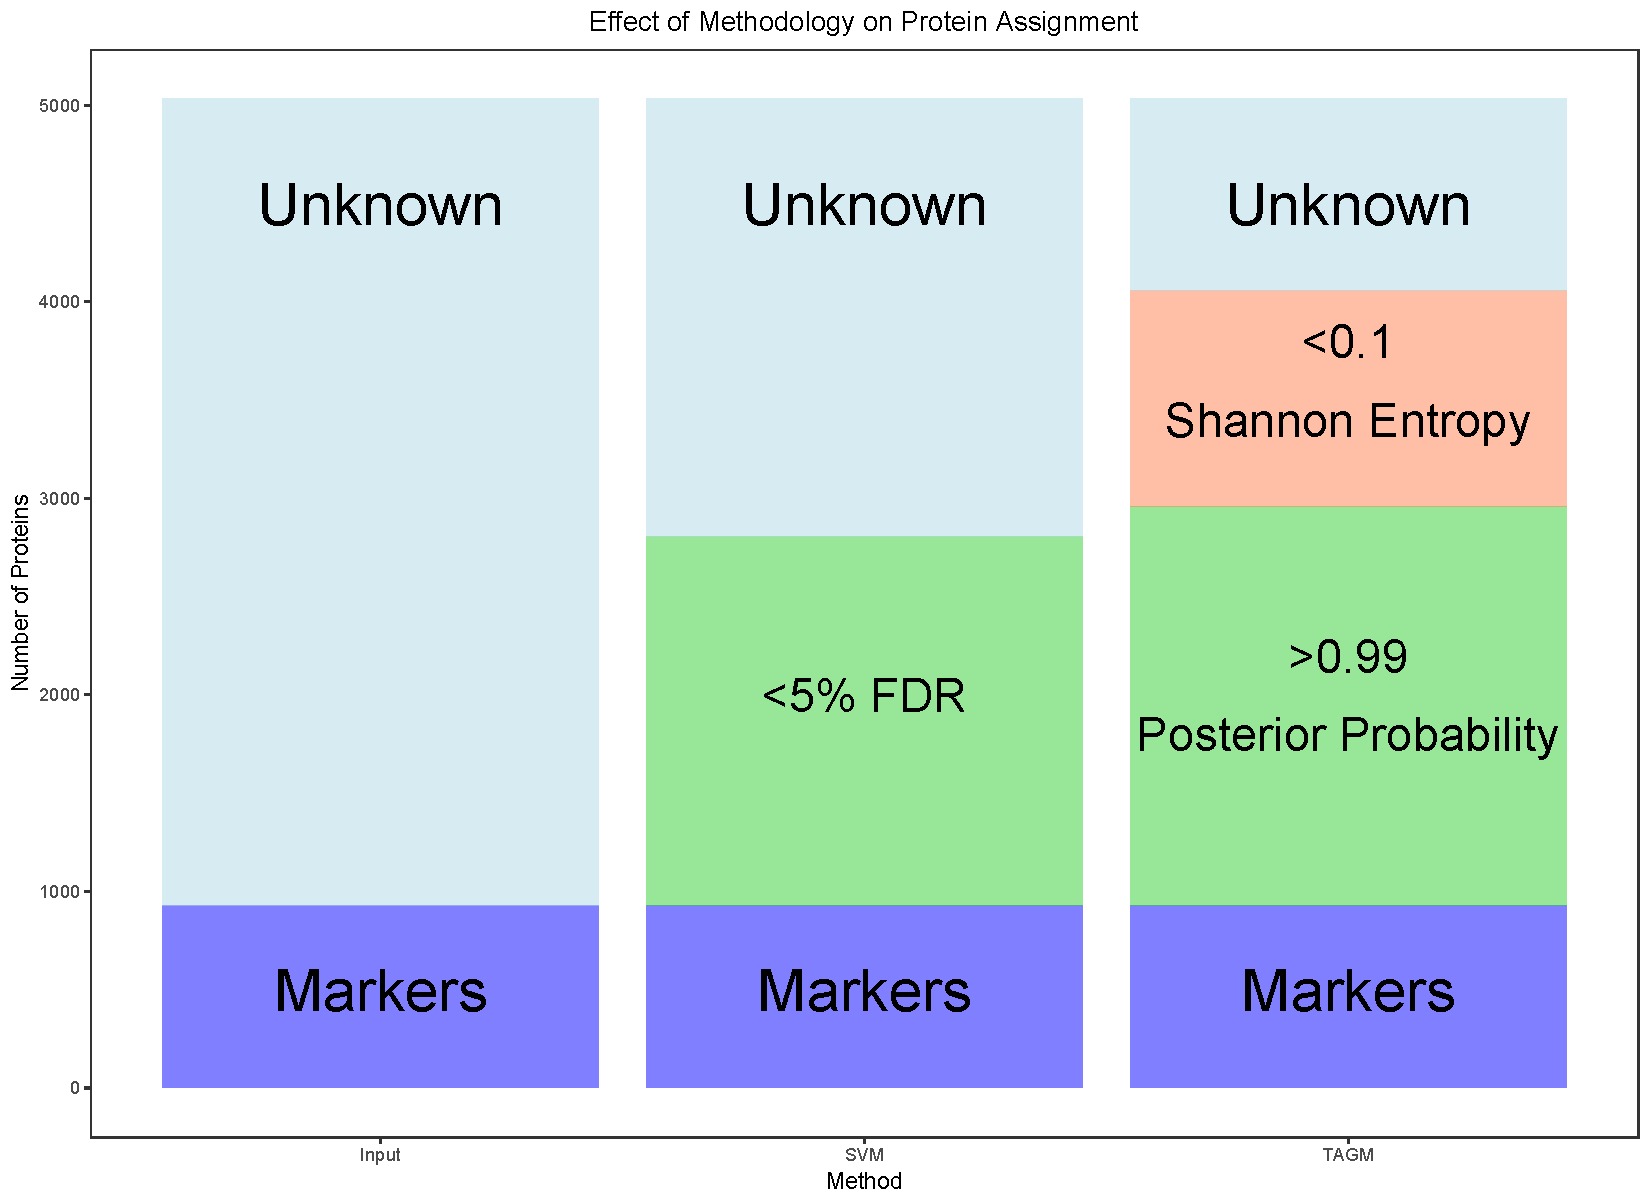
\includegraphics[width=.8\linewidth]{./figs/ConcludePlot.pdf}
  \end{figure}
\end{frame}

\begin{frame}{Multi-localisation: \textbf{localisations}}
  \begin{figure}
    \centering
    \sidebysidecaption{0.55\linewidth}{0.42\linewidth}{
      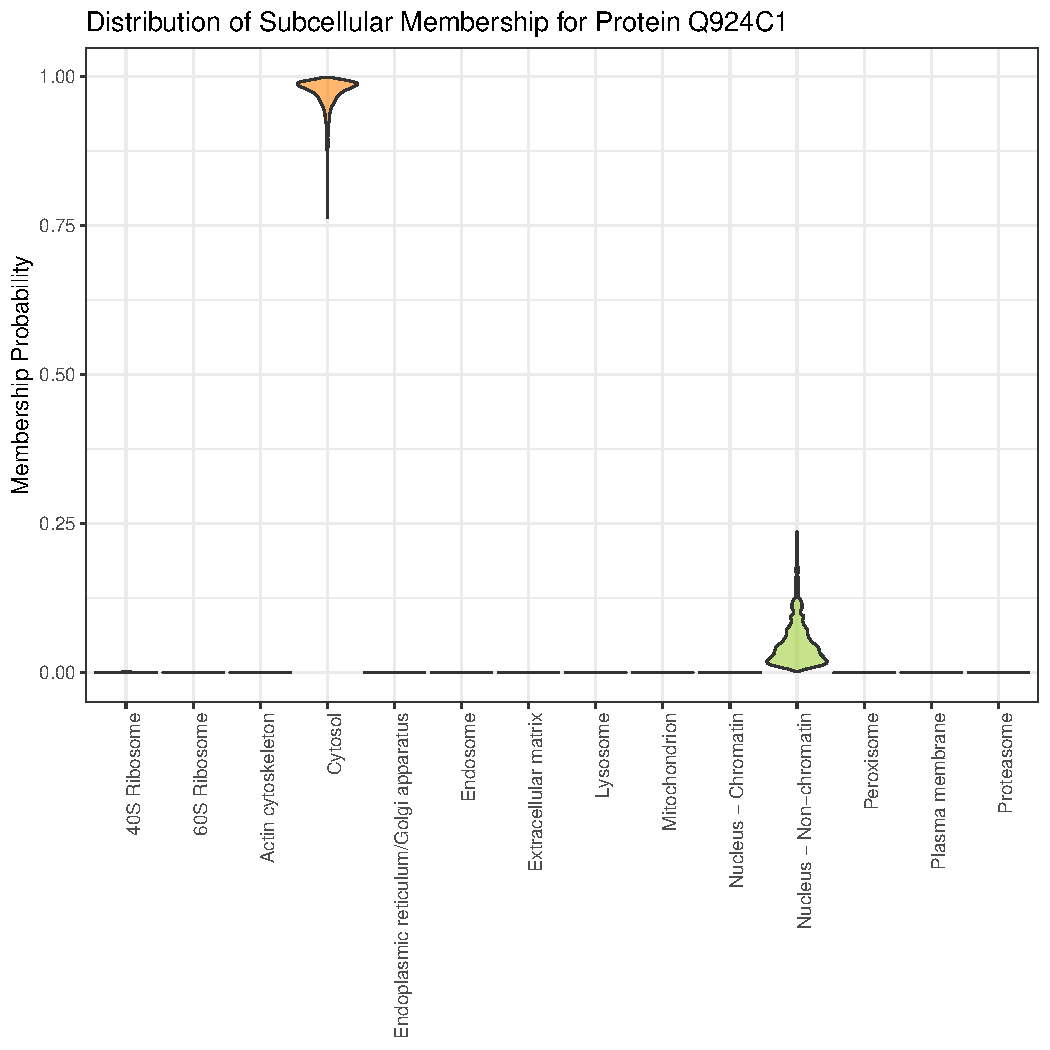
\includegraphics[width=1\linewidth]{./figs/Q924C1-prob-1.pdf}
    }{
    \caption{\scriptsize \justifying Exportin 5 (Q924C1) forms part of
      the micro-RNA export machinery, transporting miRNA from the
      nucleus to the cytoplasm for further processing.  It then
      translocates back through the nuclear pore complex to return to
      the nucleus to mediate further transport between nucleus and
      cytoplasm. The model correctly infers that it most likely
      localises to the cytosol but there is some uncertainty with this
      assignment. This uncertainty is reflected in possible assignment
      of Exportin 5 to the nucleus non-chromatin and reflects the
      multi-location of the protein.}  }
    %% NOTE SVM failed to classify exportin 5 to any of the two
    %% biologically plausible locations, arguably due to the similarity
    %% of the cytosol and peroxysome, to which it got assigned.

  \end{figure}
\end{frame}


\begin{frame}{Whole sub-cellular proteome uncertainty}
  \begin{figure}
    \centering
    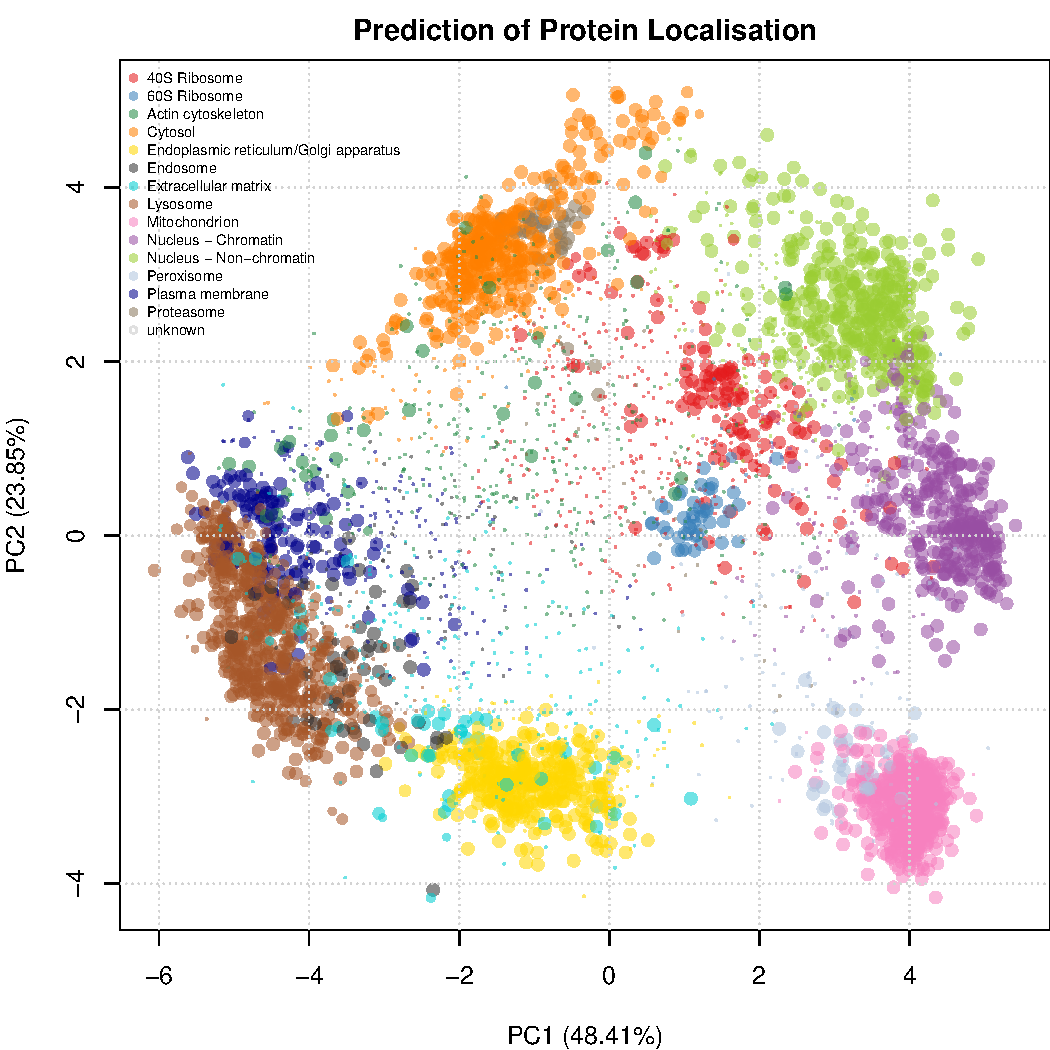
\includegraphics[width=.32\linewidth]{./figs/pca-tagm-mcmc-1.pdf}
    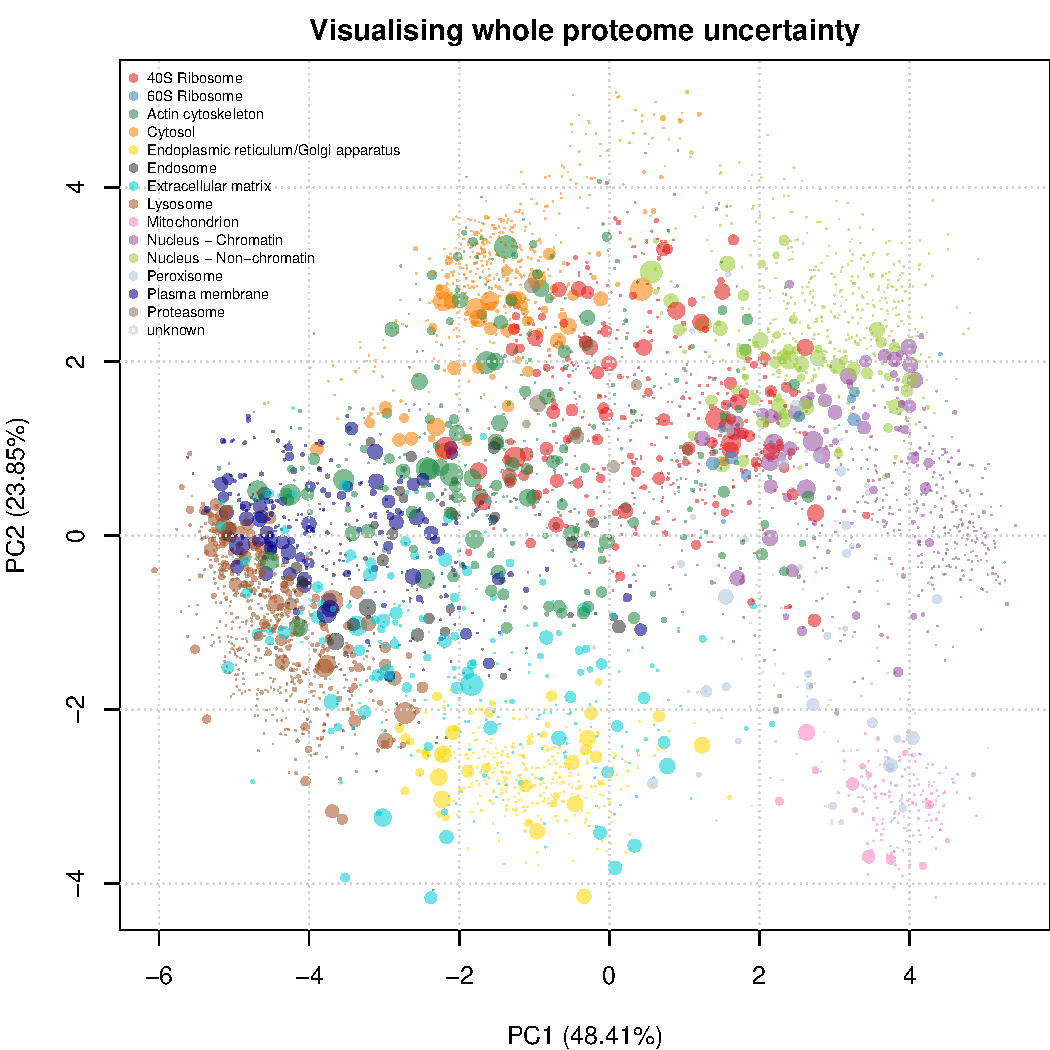
\includegraphics[width=.32\linewidth]{./figs/pca-tagm-map-1.pdf}
    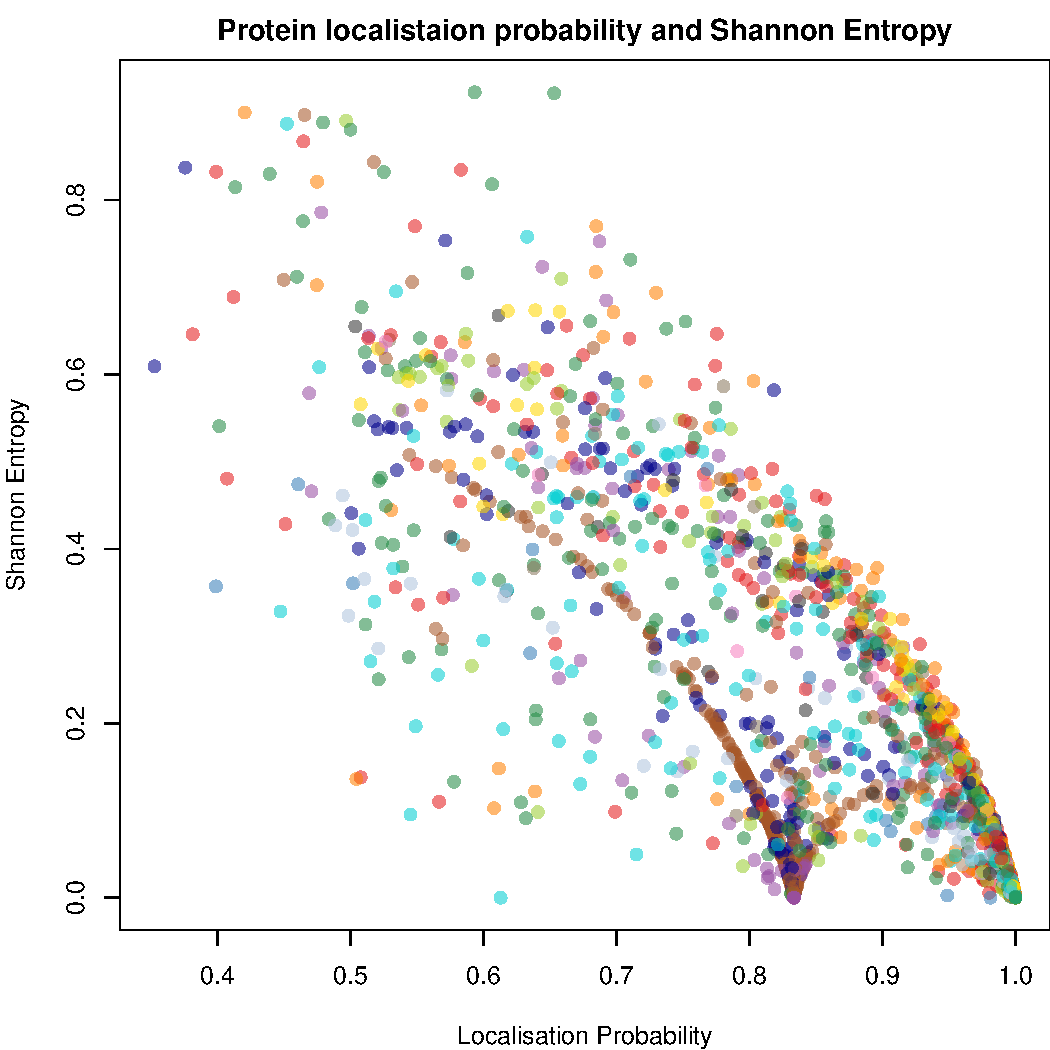
\includegraphics[width=.32\linewidth]{./figs/prob-vs-shannon-1.pdf}
  \end{figure}
\end{frame}


\section{Protein relocalisation}


\begin{frame}{Spatial dynamics}
  \begin{block}{Trans-localisation event during monocyte to macrophage
      differentiation}
    Investigate the effect of lipopolysaccharides (LPS)-mediated
    inflammatory response in human monocytic cells (THP-1)
  \end{block}

  \begin{block}{Data}
    \begin{itemize}
    \item Triplicate \textbf{temporal} profiling (0, 2, 4, 6, 12, 24
      hours).
    \item Triplicate \textbf{spatial} profiling (0 vs 12 hours) -
      early trafficking, before actual morphological differentiation
      at 24h.
    \end{itemize}
  \end{block}

  Work lead by \textbf{Dr Claire Mulvey} at the Cambridge Centre for
  Proteomics.

\end{frame}



\begin{frame}
  \begin{figure}[h]
    \centering
    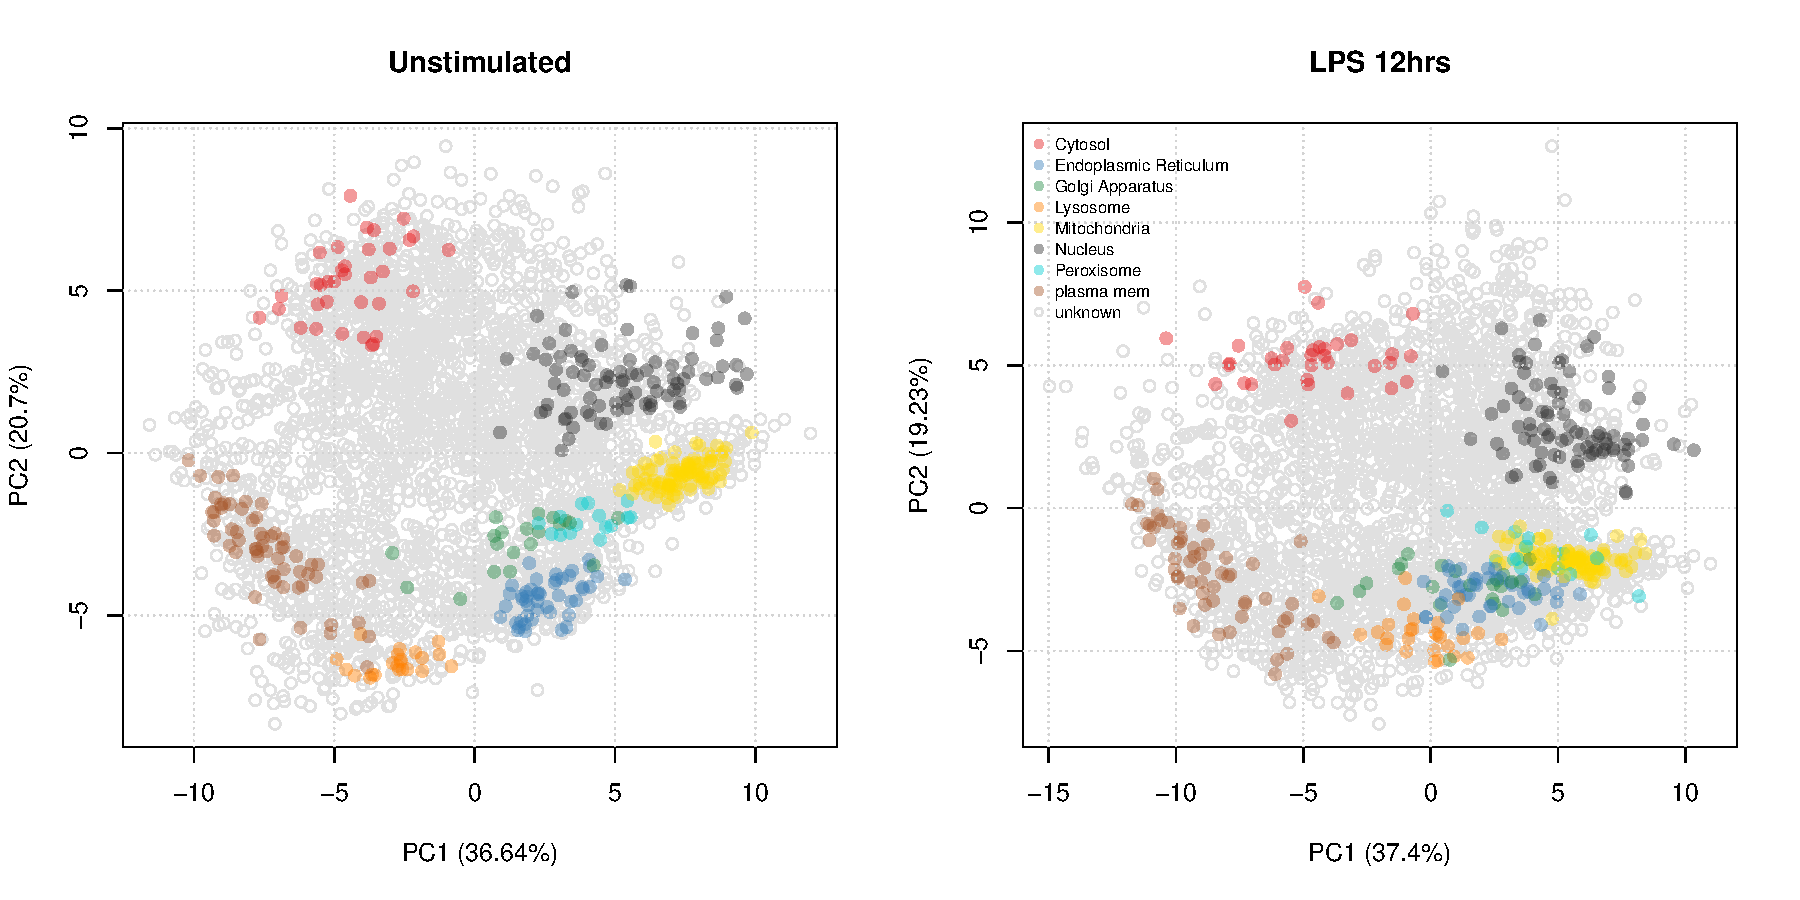
\includegraphics[width=\linewidth]{./figs/lps.pdf}
    \caption{Spatial maps of unstimulated and LPS-treated cells
      (combined triplicates).}
  \end{figure}
\end{frame}

\begin{frame}
  \begin{figure}[h]
    \centering
    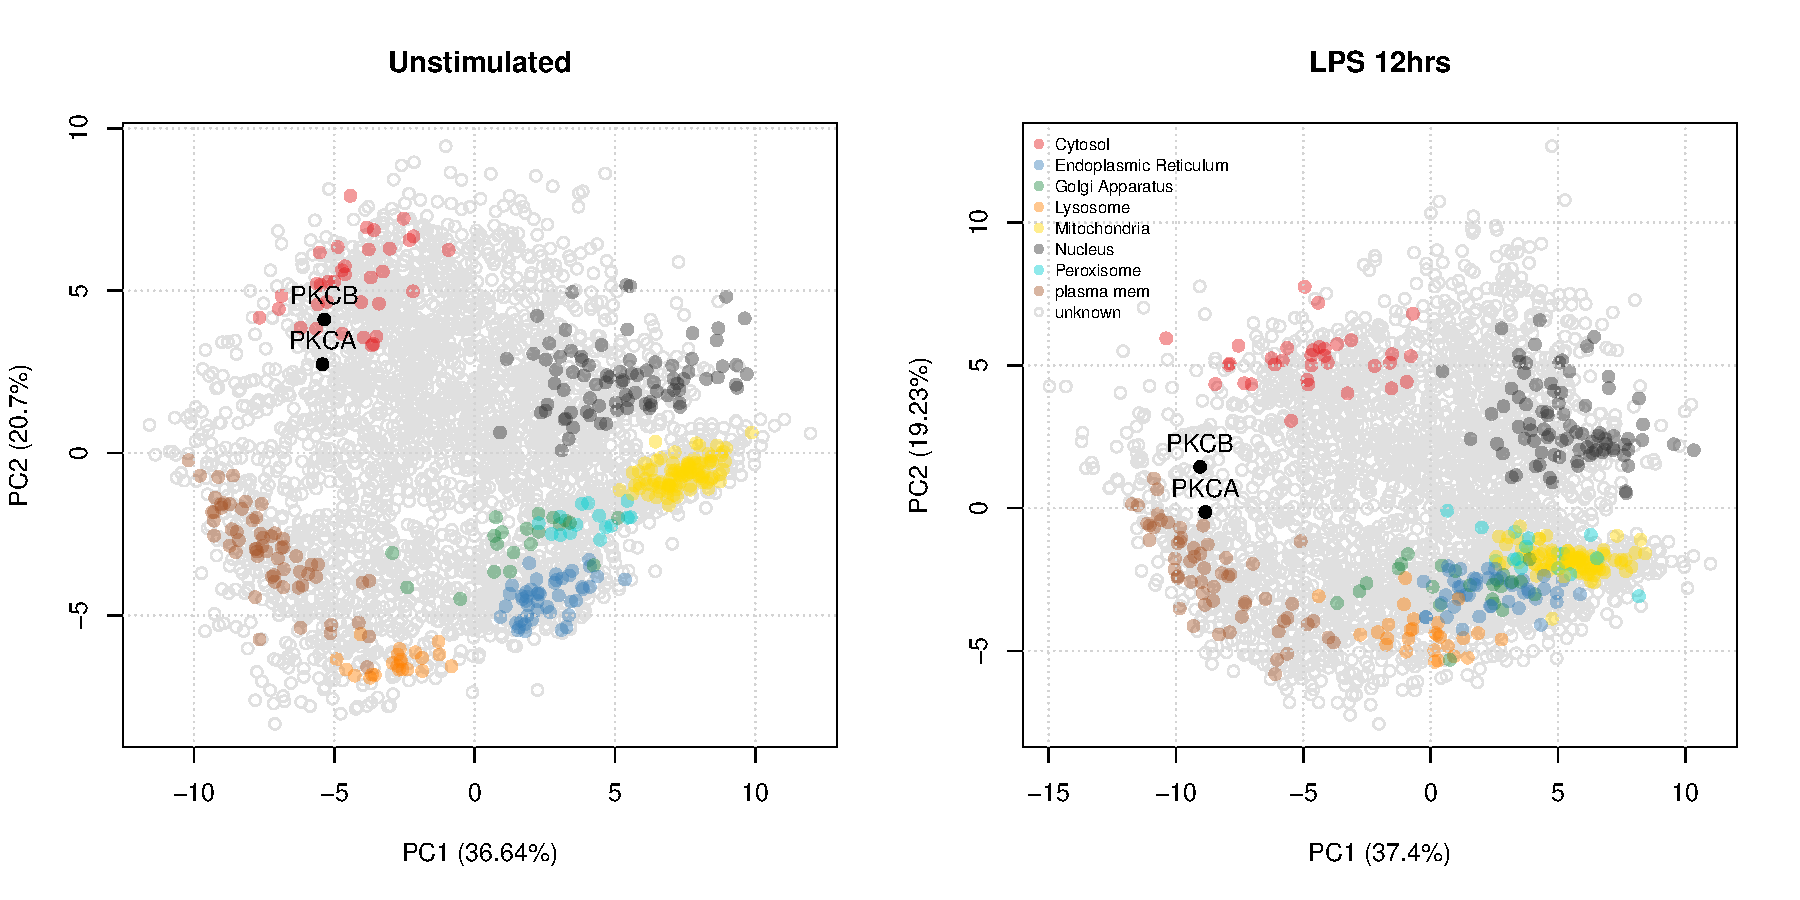
\includegraphics[width=\linewidth]{./figs/lps-pkc.pdf}
    \caption{Relocation of Protein Kinase C $\alpha$ and $\beta$ from the
      cytosol to the plasma membrane, \textbf{driving maturation into
        a differentiated macrophage phenotype}.}
  \end{figure}
\end{frame}

\begin{frame}
  \begin{figure}[h]
    \centering
    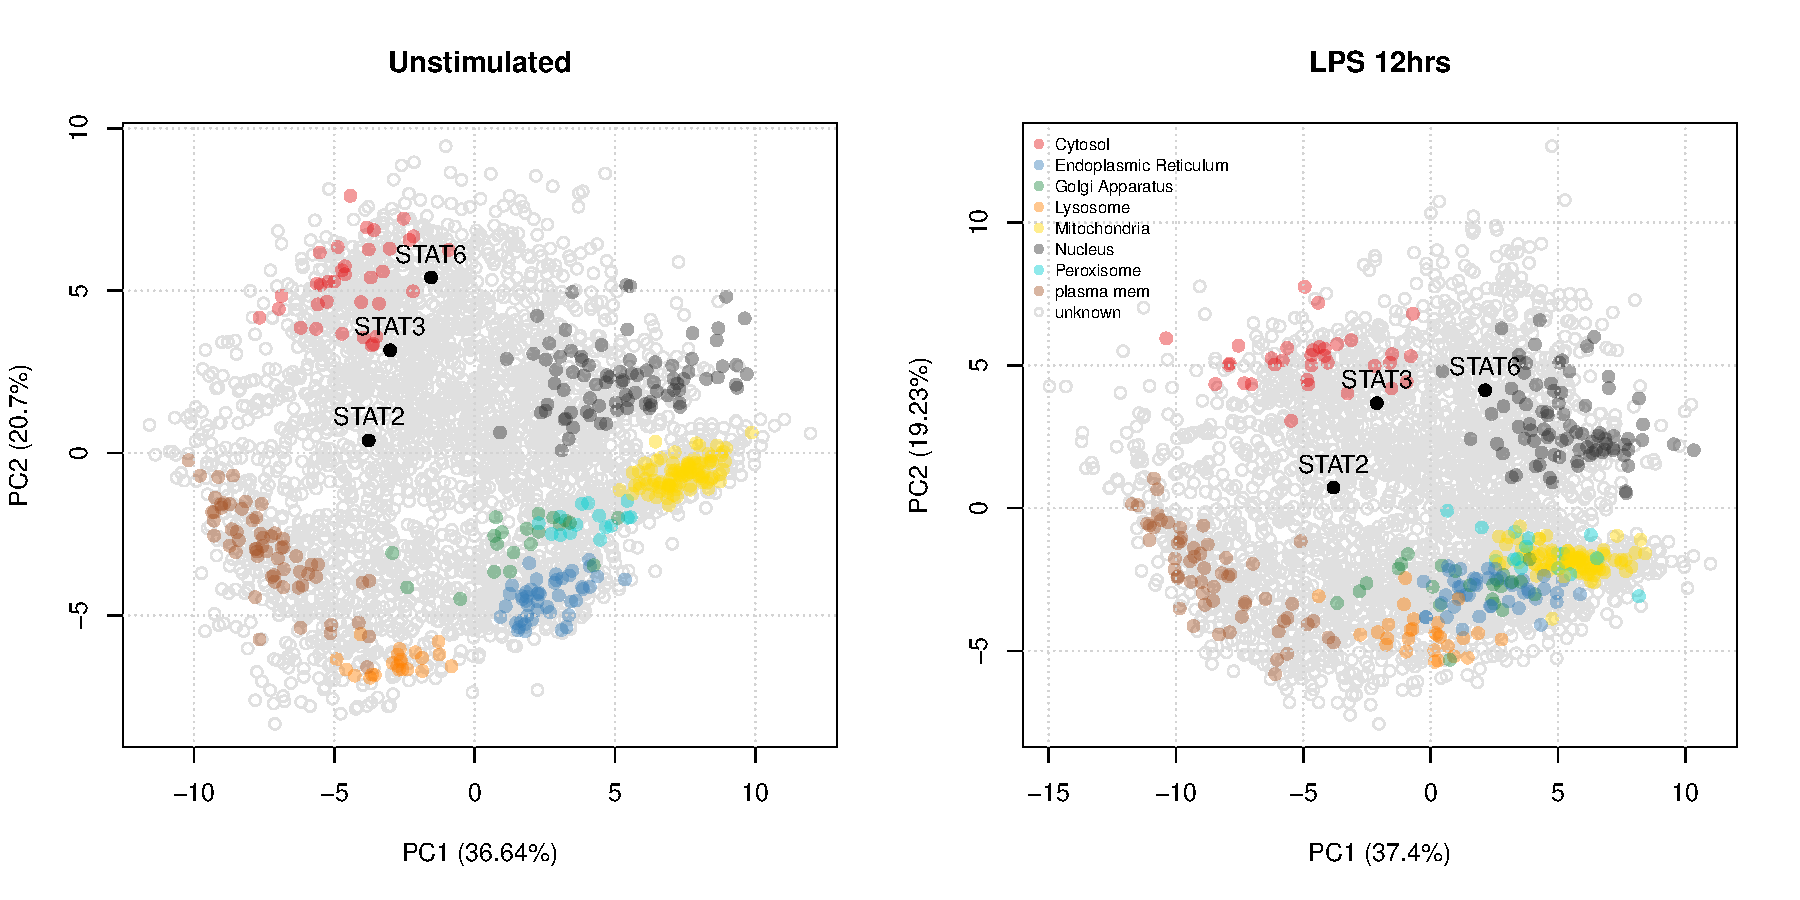
\includegraphics[width=\linewidth]{./figs/lps-stat.pdf}
    \caption{Relocation of Signal transducer and activator of
      transcription 6 (STAT6) from the cytosol to the Nucleus,
      \textbf{activating anti-bacterial and anti-viral-like
        response}. Validated by microscopy and see also
      \cite{Chen:2011}.}
  \end{figure}
\end{frame}



\begin{frame}
  \begin{block}{Folding and stability}
      \begin{itemize}
      \item Re-localisation upon protein post-translational modification (PTM).
      \item Effect of PTM on protein structure.
      \item Link between structure and localisation.
      \end{itemize}
  \end{block}
\end{frame}


\begin{frame}[fragile]{Conclusions}
  \begin{itemize}
  \item Protein sub-cellular localisation: \textit{localisation is
    function}.

  \item Reliance on computational biology, statistics and dedicated
    software (for example \texttt{MSnbase} \citep{Gatto:2012},
    \texttt{pRoloc} \citep{Gatto:2014}) to interpret data and acquire
    biological knowledge (details not shown).

  \item Rigorous computational infrastructure 
    and sound data analysis and interpretation is a \textbf{long term
      investment}.

  \end{itemize}

\end{frame}


\begin{frame}[allowframebreaks]{References}
  \scriptsize
  \bibliographystyle{plainnat}
  \bibliography{refs}
\end{frame}


\begin{frame}
  \begin{block}{Acknowledgements}
    \begin{itemize}
    \item \textbf{Mr Oliver Crook} and \textbf{Dr Lisa Breckels}, (U
      of Cambridge): spatial proteomics, machine learning, software.
    \item Funding: BBSRC (UK), Wellcome Trust (UK)
    \end{itemize}
  \end{block}

  \bigskip
  Slides: \url{http://bit.ly/20190718iscb} (CC-BY)
  \bigskip


  \begin{center}
    \textbf{Thank you for your attention}
  \end{center}

\end{frame}

\end{document}
